\subsection{Structure}\label{subsec:structure}

\subsubsection{System structure}
\textit{Replic-Read} will be split in four main system-components:
\begin{enumerate}
    \item \textbf{Browser extension} (the "active client"), implemented in AngularJS\@.
    \item \textbf{Web app} (the "passive client"), implemented in AngularJS\@.
    \item \textbf{Backend server}, implemented in Java with Spring.
\end{enumerate}

The Backend server will store data in any compatable SQL-Database.
Both clients communicate with the server via an exposed REST-API\@.

\paragraph{Responsibilities of system-components}
This section gives a better and more detailed overview of the single system components and their interfaces and dependencies.
Figure~\ref{fig:component-system} shows a component diagram of the system architecture.

\begin{figure}
    \centering
    \fbox{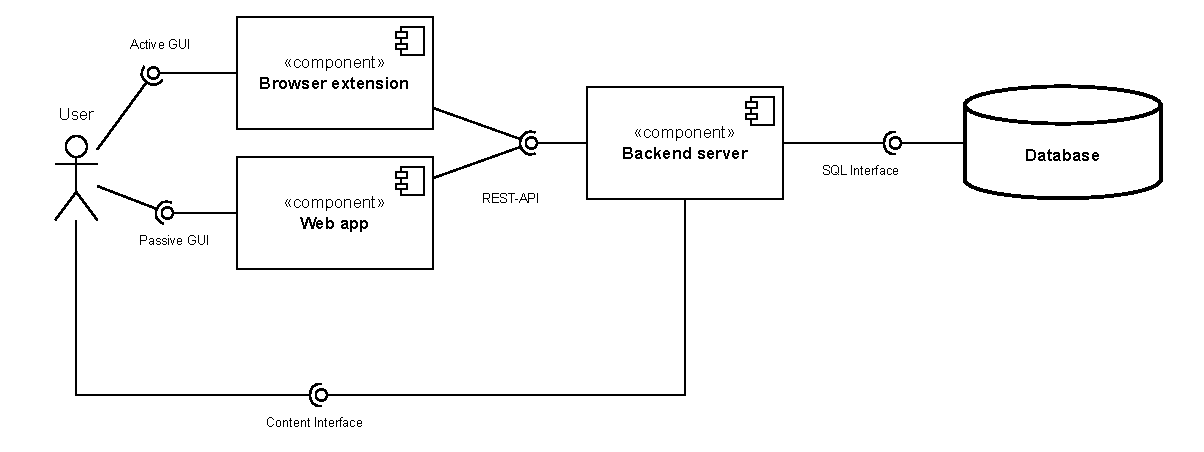
\includegraphics[width=\linewidth]{component-system}}

    \caption{Components of the system}
    \label{fig:component-system}
\end{figure}

\subparagraph{Browser extension}
The browser extension is mostly responsible for creating replics, and therefore needs to run inside the browser.
The browser extension communicates with the api provided by the browser to scrape the html-pages, and the REST-API of the backend-server for authentication and data upload.

\subparagraph{Web-app}
The web-app is the web-app that is mainly used to access shared replics, but also handle own data.
The web-app client only interacts with the REST-API provided by the backend-server.

\subparagraph{Backend server} (The "server")
The backend server acts as a middleman between the clients and the database.
It ensures data integrity, manages authentication and authorization and exposes a REST-API as means of comunication to the clients.
Additionally, the backend exposes an the \textit{Content-Interface} that allows users to view the replicated HTML of replics.

\subparagraph{Database}
The database is an external component provided by the server administrators in the form a \textit{jdbc-url} and optionally credentials.
The database stores all data and is controlled by the backend server.

\paragraph{Minimum requirements for a functioning system}
For the system to be functioning, both the server and database must be reachable, as both clients depend on the server, and the server depends on the database.
While the subsystems of the web-app and browser extension can be used independantly, the whole functionality is only available with both subsystems running: Replics can only be created on the browser extension, viewed on the server, and metadata accessed on the web-app.

\subsubsection{Deployment}
The deployment of the system happens on several devices: clients are deployed on the user device inside the browser, whereas server and database are deployed on other, not necessarily the same, device.
Figure~\ref{fig:deployment} shows a deployment-diagram of the system.
While the database is technically an external component, listing it as part of the system for deployment purposes makes sense.

\begin{figure}
    \centering
    \fbox{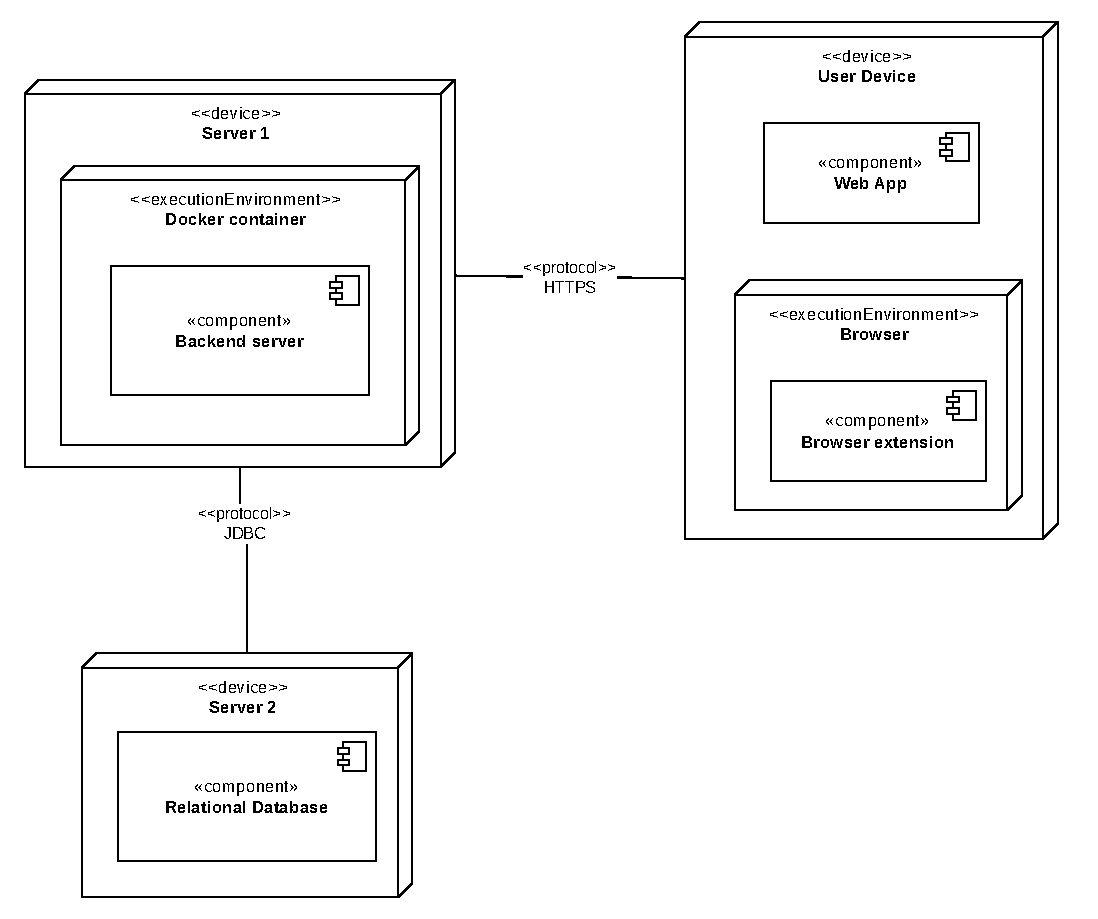
\includegraphics[width=\linewidth]{deployment}}

    \caption{Deployment of the system}
    \label{fig:deployment}
\end{figure}

\paragraph{Server deployment}
The server will be provided as a docker image \footnote{https://www.docker.com/}, that will hosted on the Github container registry \footnote{https://docs.github.com/de/packages/working-with-a-github-packages-registry/working-with-the-container-registry} for usage with docker or docker-compose.
This docker container will receive required server configuration, namely the connection to the database and the domains the system is installed on.
The docker container will expose one port, on which the REST-API and Content-Interface will be accessible.
Routing incoming requests over the domain into the container, as well as SSL-setups are the responsibility of the system admin. \newline
Deploying the server as a docker container allows great flexibility and adaptability into existing docker setups, one of the largest deployment systems.

\paragraph{Web client deployment}
Like the server, the web client will also be provided as a docker image, that will be hosted on the Github container registry.
This docker container will receive configuration, namely a URL to the bacend-server, via the environment variables.
The container will expose one port, on which the web-app will be accessible.
Routing incoming requests over the domain into the container, as well as SSL-setups are the responsibility of the system admin. \newline

\paragraph{Browser extension deployment and distribution}
The Browser extension will be distributed over the Chrome Web Store \footnote{https://chromewebstore.google.com/} and the Mozilla Addons Portal \footnote{https://addons.mozilla.org/de/firefox/}.
Safari ist not supported.
Users will be able to download the extensions and use them.

\subsection{Architecture}\label{subsec:architecture}

\subsubsection{Client-Server Architecture}
The system is based on a client-server architecture.
The server controls the database, that is the single-source-of-truth for the state of the system. \newline
Unlike traditional client-server systems, Replic-Read provides two clients to the user.
This is required due to technical constraints. \newline
Furthermore, the backend server exposes the Content-Interface that is to be accesses by the user directly without a client as middleware.

\subsubsection{Hexagonal Architecture}
The \textbf{Hexagonal Architecture} \footnote{https://en.wikipedia.org/wiki/Hexagonal\_architecture\_(software)} in an architecture pattern that implements ideas of Domain-Driven-Design.

\paragraph{Domain}
The \textbf{Domain} is at the center of the application.
It should be as independant of frameworks, libraries and technologies as possible, has almost no external dependencies and no internal dependencies.
The \textbf{Domain} provides primary ports, and declares secondary ports.

\paragraph{Ports}
\textbf{Ports} are means of communication of the \textbf{Domain}.
Primary (\("\)driving\("\)) ports are provided by the \textbf{Domain} and used to provide the interface layer.
Secondary (\("\)driven\("\)) ports are declared and used by the \textbf{Domain}.
They are implemented by the infrastructure layer.

\paragraph{Infrastructure Layer}
The \textbf{Infrastructure Layer} implements the secondary ports from the \textbf{Domain}.
These implementations communicate with external services like a database, email provider or storage system.

\paragraph{Interface Layer}
The \textbf{Interface Layer} implements external interfaces like REST-APIs, CLI's etc.
It uses the primary ports defined by the \textbf{Domain}.

\subsubsection{Model-View-ViewModel}
The Model-View-ViewModel \footnote{https://de.wikipedia.org/wiki/Model\_View\_ViewModel} (short \textbf{MVVM}) is a common pattern to decouple elements in systems with a GUI\@.
This pattern will be used in both, the web-client and the browser-extension.
Below is an explanation of all three components \textbf{Model}, \textbf{View} and \textbf{ViewModel}.

\paragraph{View}
The \textbf{View} describes the visualization of the data.
It communicates with the \textbf{ViewModel} by sending user events, and receiving state.
In AngularJs, the \textbf{View} is represented by the HTML-template.

\paragraph{ViewModel}
The \textbf{ViewModel} acts as the middleman between the \textbf{View} and the \textbf{Model}.
It manages the state for one \textbf{View} and reacts to events from it.
To update the state it can query data or be notified of changes from the \textbf{Model}.
In Angular, the \textbf{ViewModel} is represented by the component class.

\paragraph{Model}
The \textbf{Model} is responsible for the data.
It prepares the data from the data sources in such a way that it is usable in the \textbf{ViewModel}.
In Angular, the \textbf{Model} is represented by the services.

\subsubsection{Clients structure}
Both clients (passive and active) will be implemented using \textit{AngularJs}.
The component pattern that is enforced by AngularJS is closely related to the \textbf{MVVM} pattern, as explained below:
\begin{itemize}
    \item The \textbf{View} corresponds to the \textit{HTML-template} that defines the DOM-structure.
    \item The \textbf{ViewModel} corresponds to the \textit{Controller} class.
    \item The \textbf{Model} corresponds to the \textit{Service} classes that are injected into the ViewModel
\end{itemize}

\paragraph{Model structure}
The model of each client consists of the shared model, and a model specific to that client.
\begin{enumerate}
    \item \textbf{Shared model}: Exposes domain-models, data services and authentication logic.
    \item \textbf{Specific model}: Exposes specific logic for each client.
    See more below.
\end{enumerate}
This allows to share logic that both clients need, namely authentication logic and domain models, but also have specific logic that is decoupled from the other client.

\subsubsection{Server structure}
The server will utilize a Hexagonal architecture, where the interface layer deals with exposing the \textbf{REST-API} and \textbf{Content Interface}, the Domain handles the domain logic and the infrastructure layer will handle communication to the database, filesystem and email-provider.

\paragraph{Interface Layer}
The interface layer will expose the \textbf{REST-API} and \textbf{Content-Interface}.
To do so, it will utilize the domain rules provided by the domain.

\subparagraph{REST-API}
The REST-API is the api that the web-client and browser extension will communicate with.
Splitting the request-procedures in a \textbf{Request-Executor} and \textbf{Request-Dispatcher} is a common practice to isolate the HTTP-Endpoints from the actual calls to the domain.
This interface also handles access-control, authorization and authentication.

\subparagraph{Content Interface}
The Content interface is a direct access to the replicated HTML-filesa user creates when a replic is created.
This is done in a form of a minimal REST-API that takes an id of the replic and returns the raw html.

\paragraph{Domain}
The domain exposes services for the different parts of the system.
These are accessed by the \textbf{Request-Executor}.

\paragraph{Infrastructure Layer}
The infrastructure layer implements the secondary ports from the domain, that handle access to the \textbf{Database}, \textbf{Filesystem} and \textbf{Email-provider}.

\subparagraph{Database}
The \textbf{Database} part defines entities and queries to connect to the database.
It implements the secondary ports of the domain, which in this case are repositories for the several entities and their relations.

\subparagraph{I/O}
The \textbf{I/O} part gives a high-level access to the internal filesystem that is needed to save the replicated HTML-files for a replics.
These can't (or shouldn't) be stored in a relational database, which is why we need this abstraction to the local filesystem.

\subparagraph{Messaging}
To verify a user's email address, an email is sent to that address.
To encapsulate the logic of sending the email, this component is needed.

\subsubsection{Authentication}
Authentication in Replic-Read happens only via credentials.
Logging in creates a \textit{JWT} \footnote{https://www.jwt.io/} (the "access-token") and a refresh-token.

\paragraph{Access token}
The access token must be provided for every request to either of the API's.
It is used to validate the user's identity and bind a request to a specific account.
Access tokens have a short lifespan of a few minutes and can't be invalidated.

\paragraph{Refresh token}
Refresh tokens are used to re-login the user if an access-token was invalid or expired without prompting the user to re-enter their credentials.
Refresh tokens have a much longer lifespan of several days and can be invalidated.
A reference to each refresh-token is saved in the database to keep track.

\subsubsection{Example Interaction}
To explain the interaction of the different system components and their own component, we show a sequence-diagram that shows the interaction for the \textit{Create-Replic} product feature. \newline
Figure~\ref{fig:sequence-create-replic-client} shows the interactions on the active client, after the user configured the replic and clicked the \("\)Create Replic\("\) button. \newline
Figure~\ref{fig:sequence-create-replic-server} shows the interactions on the server, after the server received the HTTP-request to create a new replic.

\begin{figure}
    \centering
    \fbox{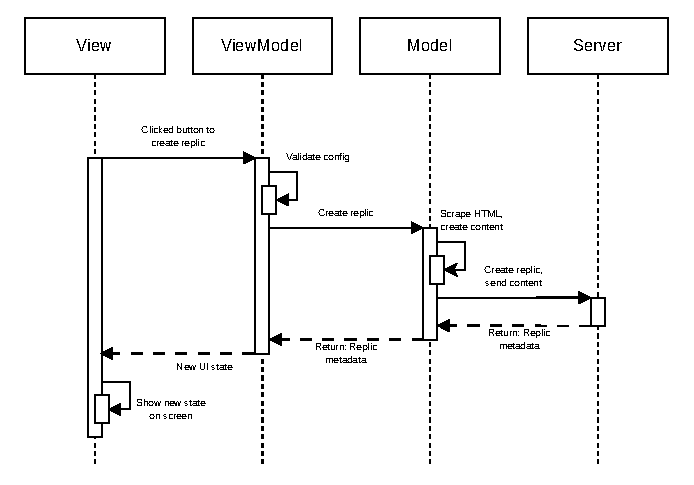
\includegraphics{sequence-create-replic-client}}
    \caption{Example interaction for create-replic on the active client}
    \label{fig:sequence-create-replic-client}
\end{figure}

\begin{figure}
    \centering
    \fbox{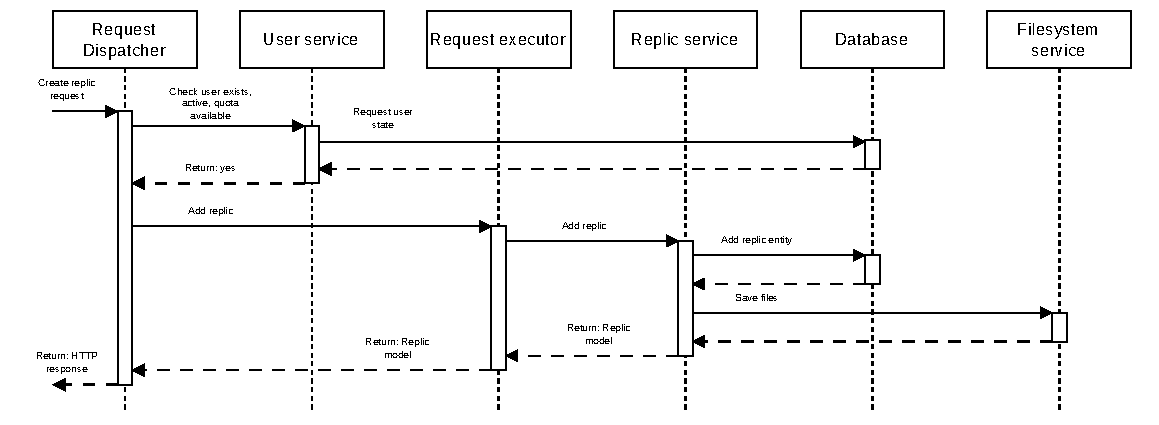
\includegraphics[angle=90]{sequence-create-replic-server}}
    \caption{Example interaction for create-replic on the server}
    \label{fig:sequence-create-replic-server}
\end{figure}

\subsection{Component specification}\label{subsec:component-specification}

\subsubsection{Clients}

\paragraph{Shared model}
Due to the same Implementation and similar objectives, some domain logic is required by both clients, which can essentially be reduced to Authentication and Replic-Creation.
To prevent multiple logic, we decided to have a shared model that contains the common requirements.
We also decide to let the \textbf{Shared Model} be responsible for all the client-logic that does not depend on the specific execution environment.
For example, a service that exposes functionality to list the users replics may be part of the \textbf{Shared Model}, despite not being used in the active client.
This way, we gain flexibility for possible future expansion. \newline
Figure~\ref{fig:component-clients-shared} shows the inner structure and provided interfaces of the \textbf{Common Model}:
The main components are the \textit{Services} and \textit{Authentication} components.
These expose logic for authenticating and getting data from the server.
The \textit{Services} component dpeends on the \textit{Authentication} component to perform authentication when fetching user-specific data.
Both dpeend on the \textit{NetworkClient} and \textit{Domain} component, that provide functionality to perform web-requests and the domain-models.
The \textit{Authentication}, \textit{Domain} and \textit{Services} component are bundles in a \textit{Facade} and provided to the \textbf{Active Client} and \textbf{Passive Client}.

\begin{figure}
    \centering
    \fbox{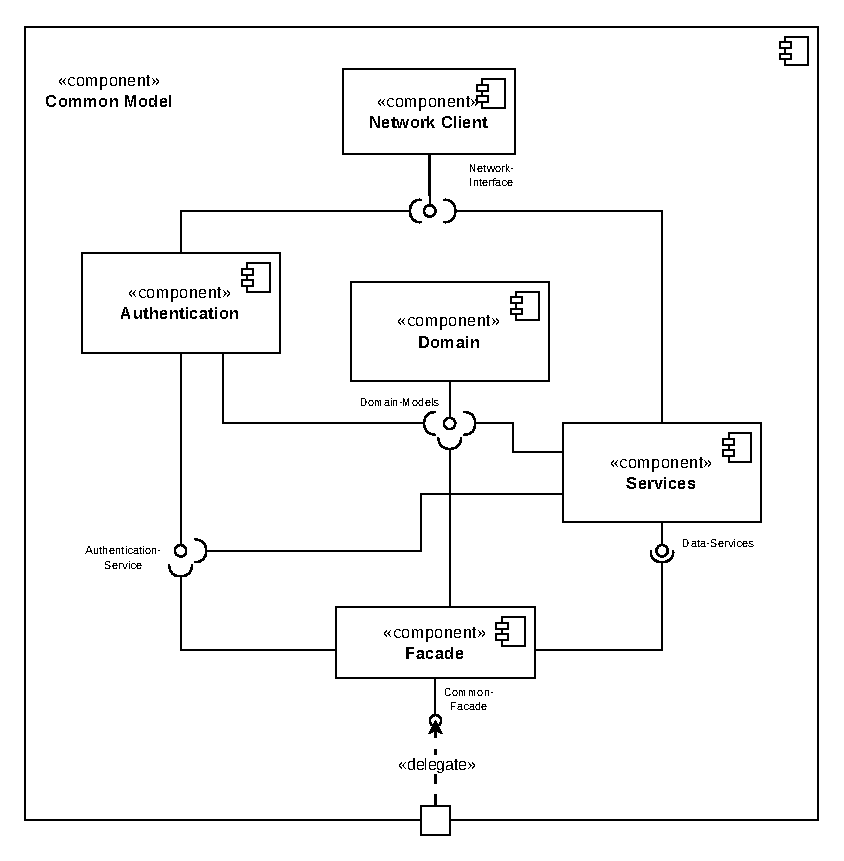
\includegraphics[width=\linewidth]{component-clients-shared}}
    \caption{Components of the shared client model}
    \label{fig:component-clients-shared}
\end{figure}

\paragraph{Active client}
Figure~\ref{fig:component-clients-active} shows the inner structure of the \textbf{Active Client}: The active client depends on the shared model, and additionally has the \textit{Active Model} that provides logic specific for the active-client.
Both the shared model and active model are depended on by the \textbf{ViewModel}.
The \textbf{ViewModel} itself depends and is depended on by the \textbf{View} to expose state and event handlers, while it consumes the events fired by the \textbf{View}.

\begin{figure}
    \centering
    \fbox{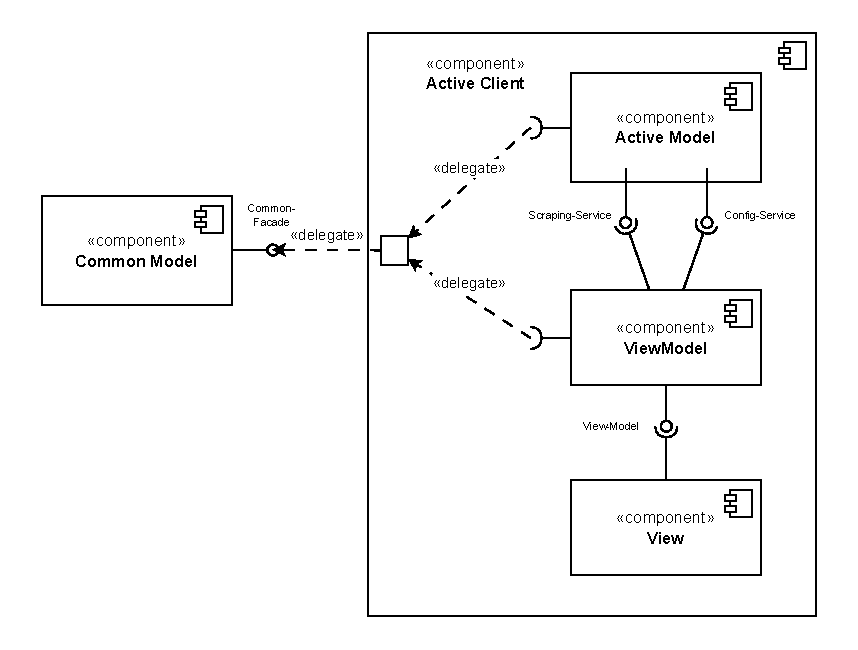
\includegraphics[width=\linewidth]{component-active-client}}
    \caption{Components of the active client}
    \label{fig:component-clients-active}
\end{figure}

\paragraph{Passive client}
Figure~\ref{fig:component-clients-passive} shows the inner structure of the \textbf{Passive Client}: The passive client depends on the shared model, and does not have an own model like the active client.
If this becomes necessary in the future, expansion is flexible.
Like in the active client, the \textbf{ViewModel} depends and is depended on by the \textbf{View} to expose state and event handlers, while it consumes the events fired by the \textbf{View}.

\begin{figure}
    \centering
    \fbox{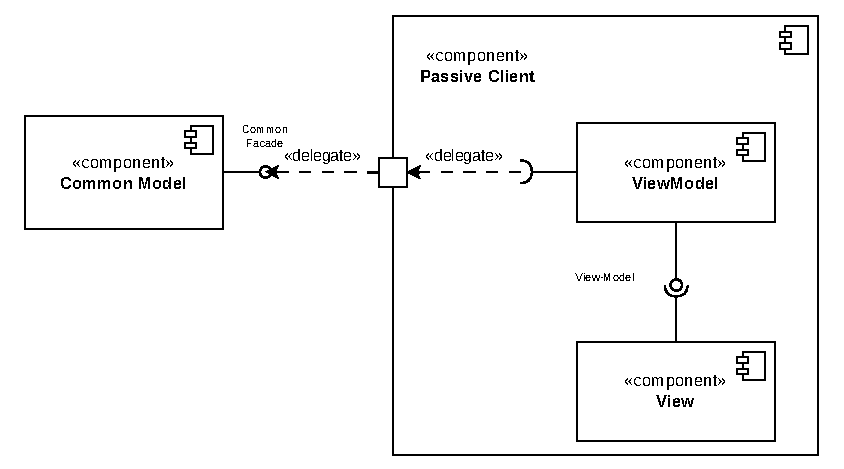
\includegraphics[width=\linewidth]{component-passive-client}}
    \caption{Components of the passive client}
    \label{fig:component-clients-passive}
\end{figure}

\subsubsection{Server}
As mentioned before, the server is built in a hexagonal architecture.
Figure~\ref{fig:component-server} shows the three layers:
\begin{itemize}
    \item The \textbf{Interface Layer} exposes the REST-API for communication with the clients, and the Content-Interface for users to vew replic content.
    It consists of the \textbf{Request Dispatcher} that delegates requests to the \textbf{Request Executor}.
    There, requests are executed by using the primary ports and authorized using the \textbf{Authorizer}.
    \item The \textbf{Domain} is explained further in~\ref{par:domain}.
    \item The \textbf{Infrastructure Layer} handles direct communication with external services, namely the \textit{Filesystem}, the \textit{Database} and the \textit{Mail provider}.
    It implements the secondary ports that are required from the \textbf{Domain}.
\end{itemize}

\begin{figure}
    \centering
    \fbox{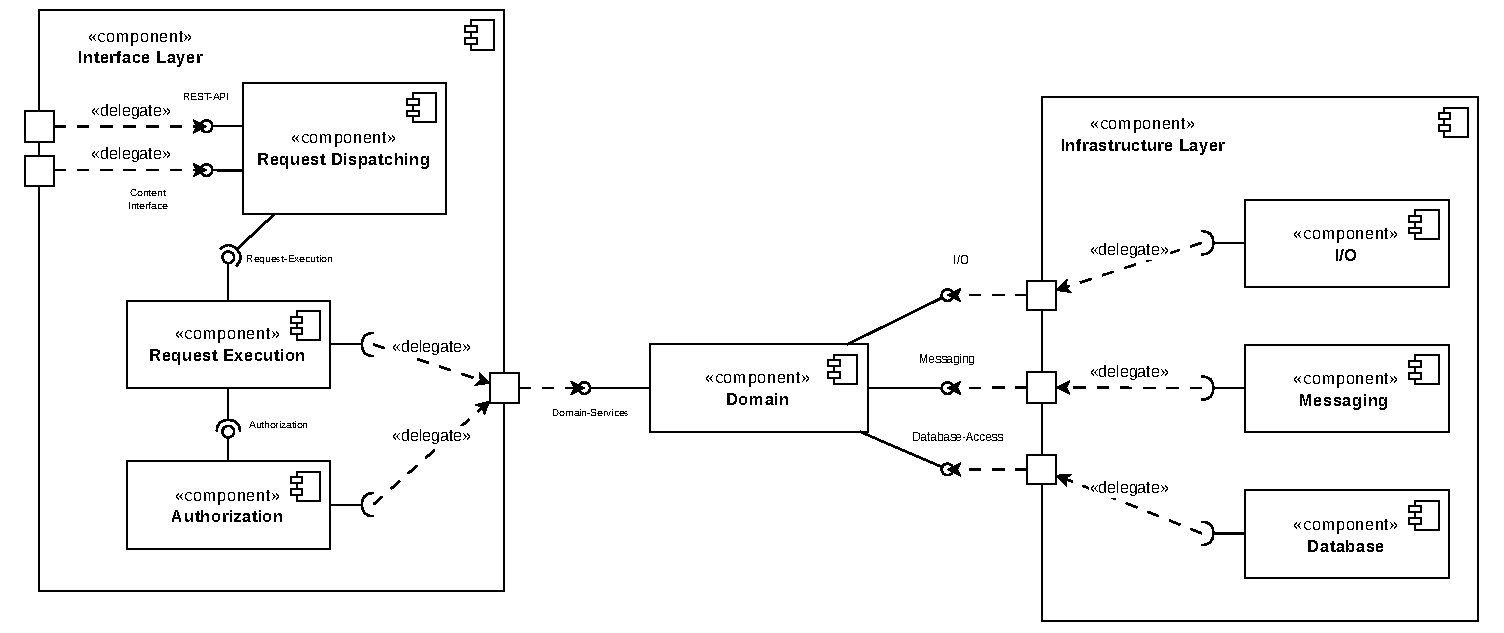
\includegraphics[width=\linewidth]{component-server}}
    \caption{Components of the server}
    \label{fig:component-server}
\end{figure}

\paragraph{Domain}\label{par:domain}
The \textbf{Domain} is the component at the center of a hexagonal architecture.
At it's heart are the domain models, as shown in Figure~\ref{fig:component-domain-models}.
They model business entities that are used throughout the application. \newline
Around the business Models, the \textbf{Domain} module declares primary and secondary ports.
Primary ports are domain services that get exposed to the \textbf{Interface Layer}, whereas secondary ports are interfaces to be implemented by the \textbf{Infrastructure Layer}.
The domain models are also exposed to all sides.
See also Figure~\ref{fig:component-domain}

\begin{figure}
    \centering
    \fbox{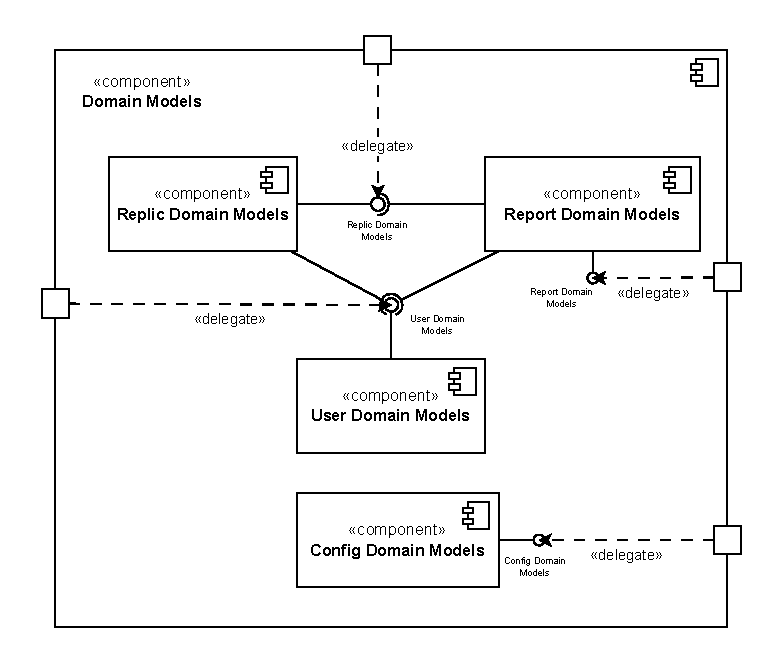
\includegraphics[width=\linewidth]{component-domain-models}}
    \caption{Components of the domain models}
    \label{fig:component-domain-models}
\end{figure}

\begin{figure}
    \centering
    \fbox{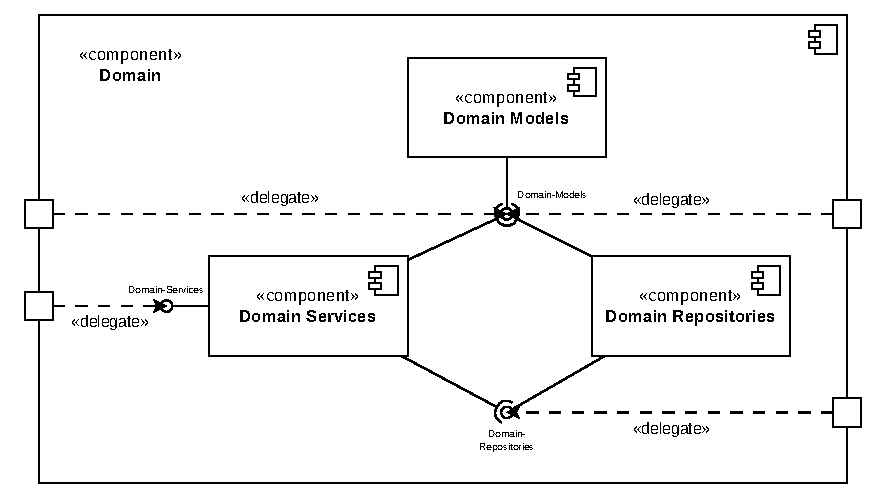
\includegraphics[width=\linewidth]{component-domain}}
    \caption{Components of the domain}
    \label{fig:component-domain}
\end{figure}

\subsection{Interface Specification}\label{subsec:interface-specification}

\subsubsection{Database Schema}
The database schema is the schema that is expected from the database that is provided.
If the database has no schema, this specified one will be loaded into the database. \newline
For the schema declaration, PostgreSQL \footnote{https://www.postgresql.org/} syntax is used.
The types \texttt{user\_state}, \texttt{replic\_state}, \texttt{media\_mode}, \texttt{auth\_user\_group}, \texttt{token\_type} \texttt{report\_state} are defined as enumerations. \newline
Figure~\ref{fig:database-schema} shows the schema visualized.
Every table has an \texttt{id} and \texttt{created\_timestamp} column that hold the UUID and creation timestamp of the record. \newline
The table \texttt{replics} keeps the basic attributes of one specific replic, and holds a reference to the author, if it was created by an account.
The tables \texttt{users} and \texttt{reports} store attributes of users and reports, where a report has a reference to the target replic, and possibly to the author of the report.
\texttt{replic\_accesses} models an access to a specfic replic, possibly with reference to the account.
In \texttt{auth\_tokens}, miscellaneous tokens related to authentication are stored, e.g.\ refresh tokens or email-verification-tokens.
The \texttt{server\_config} stores the server configuration.

\begin{figure}
    \centering
    \fbox{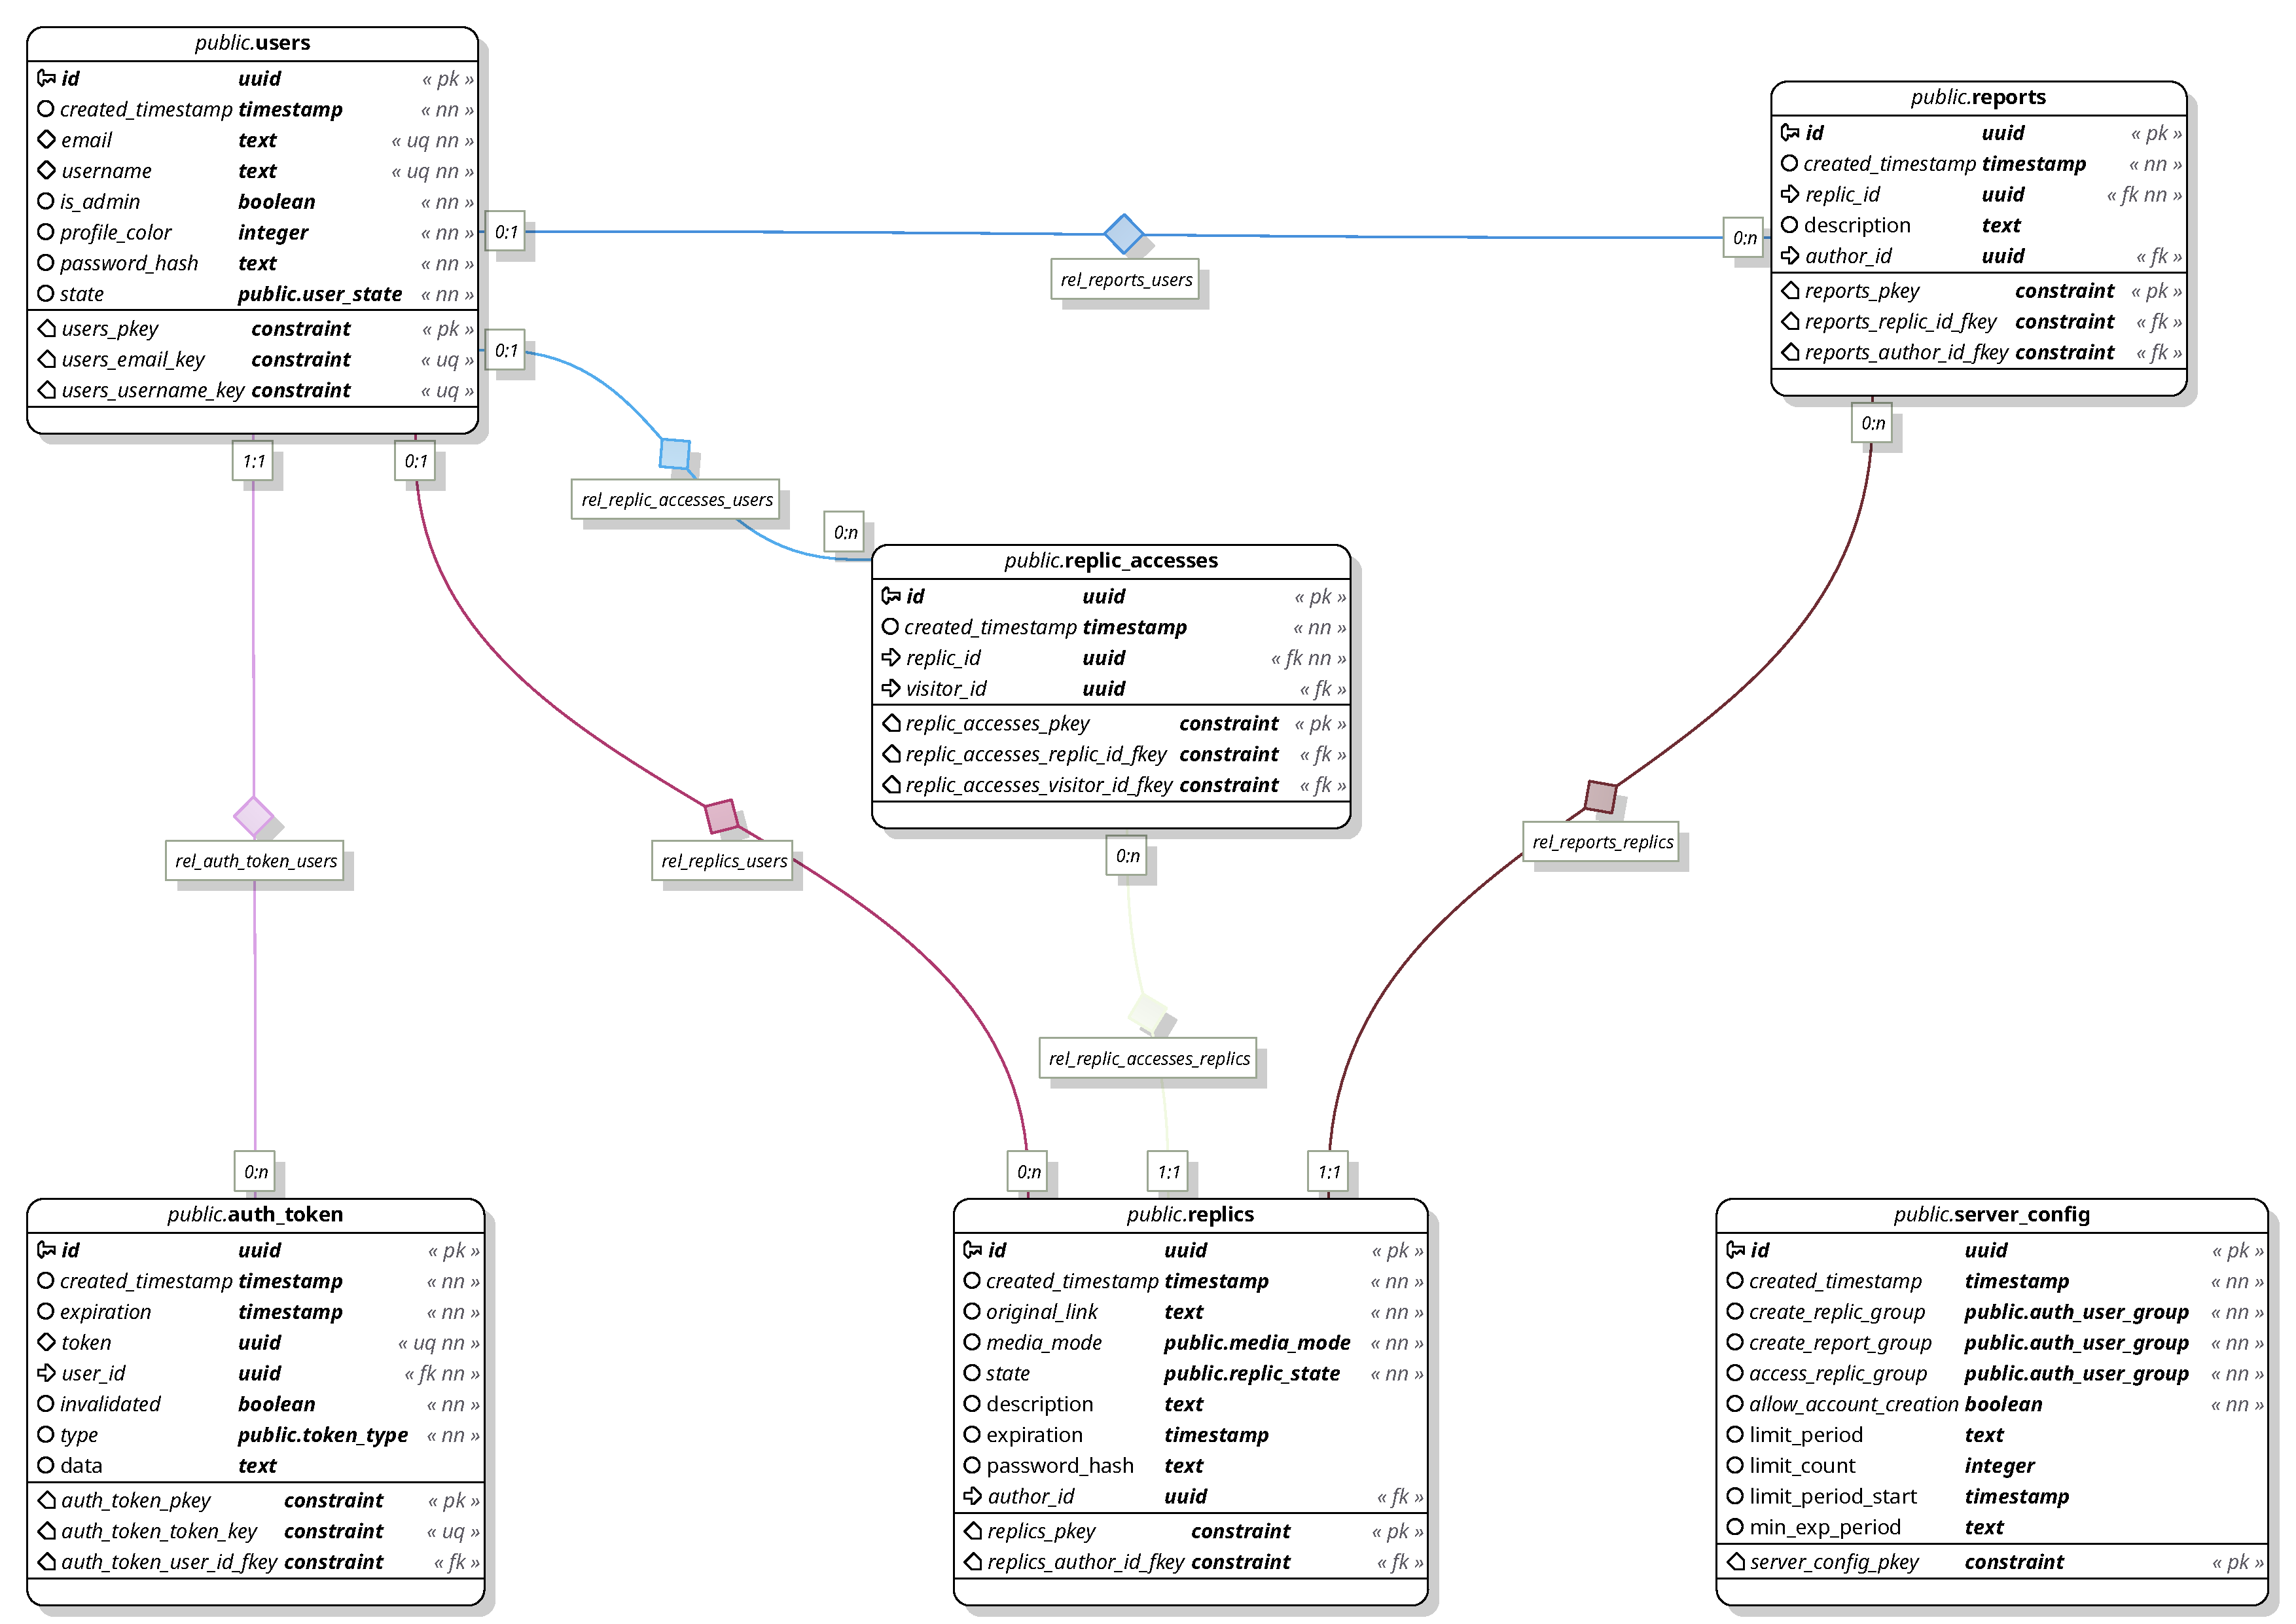
\includegraphics[angle=90, width=\linewidth]{database-schema}}
    \caption{Database schema}
    \label{fig:database-schema}
\end{figure}

\subsubsection{REST-API}
The REST-API specification is the list of endpoints that make up the REST-API\@.
This specification was created as an OpenAPI \footnote{https://www.openapis.org/} documentation, that provides a standardized way to declare endpoints, request bodies, response bodies, path variables, query parameters and errors.
Using OpenAPI has many advantages over others:
\begin{itemize}
    \item \textbf{Visualization:} To view the specification visually and interactively, many editors, such as the Swagger-Editor \footnote{https://editor.swagger.io/} are available.
    \item \textbf{Manual Testing:} Many http-clients that are used for manual testing of endpoints can accept an OpenAPI specification to set up the workspace.
    \item \textbf{Code-Generation:} Using the swagger-codegen tool \footnote{https://swagger.io/tools/swagger-codegen/}, the specification can automatically create stubs for the server or client in many programming languages and frameworks.
    \item \textbf{Generation from code:} Vice-versa, the OpenAPI-specification can be automatically generated from the server-side code in many frameworks.
\end{itemize}

The specification is available in the appendix as a json-file. \newline

\paragraph{Responses for bad authentication/authorization}
If an endpoint requires a client to present authentication, and no or bad authentication is presented, the endpoint will return status code \textbf{401}. \newline
If an endpoint requires specific permission, and that permission is not met, status code \textbf{403} is returned.
If an endpoint is specific to a resource, for example \texttt{/replics/\{id\}/content/}, and the resource was not found, status code \textbf{403} is also returned.
This is to safeguard unauthorized clients from detecting the existance of a specific resource by comparing \("\)unauthorized\("\) and \("\)not found\("\) responses. \newline
Note: Whether an endpoint requires authentication or specific permissions may be dynamic.
For example, a \textbf{POST} request to \texttt{/reports/} only requires authentication and permission depending on the server setting that defines which clients can create reports.

\paragraph{Endpoints}

\subparagraph{/server-config/} This endpoint is used to retrieve the current config on the server.
This needs to be exposed in order for the client to give the user an adequate experience.
It also allows admins to update the settings.

\subparagraph{/reports/} This endpoint is used to retrieve all reports that have not been closed/reviewed, only for admins.
It is also used to create new reports.

\subparagraph{/reports/\{id\}/} This endpoint is used to change the state of a specific report.

\subparagraph{/replics/} This endpoint is used to retrieve all replics.
The replics that are returned depend on the client, i.e.\ if the client is an admin or not.
The endpoint is also used to create new replics.

\subparagraph{/auth/submit-email-verification/} This endpoint is used to submit an email-verification-token that was sent to a user via email.
The client doesn't need to authenticate here.

\subparagraph{/auth/signup/} This endpoint is used to signup and create a new account.
Account data and credentials are provided via the request body.

\subparagraph{/auth/refresh/} This endpoint is used to get a new access-token from an existing refresh-token.
This is the default \("\)login\("\) clients will use to authenticate in the background.

\subparagraph{/me/} This endpoint is used to get information about the account that is associated with the authentication provided by the client.

\subparagraph{/me/quota/} This endpoint is used to get how many replics the user has created in the current limit period.

\subparagraph{/auth/login/} This endpoint is used to get a new refresh-token by authenticating with the credentials.

\subparagraph{/admin/shutdown/} This endpoint is used to schedule stopping the server.

\subparagraph{/admin/restart/} This endpoint is used to schedule a restart of the server.

\subparagraph{/accounts/} This endpoint is used to get all accounts on the server.
It is also used to create a new account.

\subparagraph{/replics/\{id\}/content/} This endpoint is used to retrieve the replicated HTML-content of the replic with it \texttt{id}.

\subparagraph{/auth/request-email-verification/} This endpoint is used to request an email-verification-token to be sent to the email of the account.

\subsubsection{Graphical User Interface}
The GUI will be implemented as provided in the requirements document.
To do so, we will use the AngularJS Framework.

\subsection{Internal server interfaces}\label{subsec:internal-server-interfaces}
In the following, we will explain the different internal interfaces of the server components that are visible in Figure~\ref{fig:component-server}.

\subsubsection{Request Executors}
Request dispatchers are responsible for executing the immediate actions that should be triggered by a call to a specific endpoint with a specific HTTP-message.
They are called as delegates by their respective Request Dispatcher.

\subsubsection{Authorizer}
The Authorizer encapsulates logic to determine whether a client is allowed to perform the requested action.
In most cases, this permission-checking boils down to either one of the following:
\begin{itemize}
    \item Checking if a user is an admin.
    \item Checking if a user owns a resource.
    \item Checking the value of a specific server setting.
\end{itemize}
The Authorizer is required to abstrahize and decouple that logic from the execution of the endpoint.

\subsubsection{Services}
The services exposed by the Domain module couple logic into single method calls.
Additional to data-querying of \textit{Replics}, \textit{Reports} and \textit{Accounts}, a service for authentication logic is also provided.

\subsubsection{Domain Models}
The Domain Models are rich data-objects that model the real-life domain objects like \textit{Account} or \textit{Replic}.
They are used throughout the whole app, especially in the services the domain exposes.

\subsubsection{File Accessor}
The File Accessor allows to query and save the replicated HTML-files for replics.

\subsubsection{Email Sender}
The Email Sender is an interface to easily send emails to specific users.

\subsubsection{Repositories}
The Repositories are accessors to the relational database that stores the data of the application. \newline
Each repository deals with one specific type of model and provides basic CRUD-functions.

\subsection{Internal client interfaces}\label{subsec:internal-client-interfaces}
In the following, we will explain the different internal interfaces of the client components that are visible in Figures~\ref{fig:component-clients-shared},~\ref{fig:component-clients-active} and~\ref{fig:component-clients-passive}.

\subsubsection{Network Interface}
The Network interface provides simple access to each endpoint on the server.
It also parses the returned bodies and encapsulates errors.

\subsubsection{Domain Models}
The Domain Models are rich data-objects that model the real-life domain objects like \textit{Account} or \textit{Replic}.
They are used throughout the whole app, especially in the services the Common Model exposes.

\subsubsection{Authentication Service}
The authentication service uses the Network Interface to perform authentication calls.
It is also responsible for storing the authentication-tokens securely in the browser.

\subsubsection{Data services}
The Data Services act as a wrapper around the Network Interface.
They cache data and use the Authentication Service to re-perform calls when a request failed due to wrong authentication.

\subsubsection{Scraping service (Active client)}
The Scraping Service is responsible for gathering the HTML-content of the target web-page.

\subsubsection{Signals, Event Handlers}
Each ViewModel exposes AngularJS Signals that act as an observable source of data.
These signals are used in the HTML-templates to show dynamic data to the user. \newline
Additionally, event handlers are exposed to the templates that receive events for user input.

\subsubsection{Config Service (Active client)}
The Config Service encapsulates saving of config. \newline
Currently, the config only contains the URL of the server endpoint.

\subsection{External Libraries and Frameworks}\label{subsec:external-libraries-and-frameworks}
\subsubsection{Framework: Spring}
The server uses Spring \footnote{https://spring.io/} as it's framework.
Spring is a java-framework that provides a foundation for many aspects, most notably for our project are \textit{dependency-injection} and the \textit{http-server} functionality.
It also eases testing, healthchecks and integration with other services.

\subsubsection{Hibernate}
Hibernate \footnote{https://hibernate.org/} is a library that allows spring to connect to external relational database.
Spring adds concise syntax with annotations to declare tables and repositories.

\subsubsection{Commons email}
The Apache Commons Email \footnote{https://commons.apache.org/proper/commons-email/} library is a library that allows to send emails from java code.
Next to simple text-emails, Commons Email supports embedded media, HTML-formatted emails and attachments.

\subsubsection{Java-Jwt}
The \textit{Java-Jwt} \footnote{https://github.com/auth0/java-jwt} is a library that simplifies dealing with JWT's in java code.
Creating, signing and parsing are handled by the library to ensure security.

\subsubsection{Framework: AngularJS}
AngularJS is the framework used for both clients. \newline
AngularJS is a component-based framework that allows to create single-page web-apps using the Model-View-ViewModel style.
Additionally, AngularJS provides strongly-coupled dependency injection which ensures dependency integrity.

\subsubsection{Angular Material}
Angular Material \footnote{https://material.angular.dev/} is a library that provides Material-Components \footnote{https://m3.material.io/} to the Angular templates.
Using Material components allows us to outsource the creation of a design-system and to use establishes rules for UI and UX.